
%%%%%%%% ICML 2018 EXAMPLE LATEX SUBMISSION FILE %%%%%%%%%%%%%%%%%

\documentclass{article}

% Recommended, but optional, packages for figures and better typesetting:
\usepackage{microtype}
\usepackage{graphicx}
%\usepackage{subfigure}
\usepackage{booktabs} % for professional tables

% hyperref makes hyperlinks in the resulting PDF.
% If your build breaks (sometimes temporarily if a hyperlink spans a page)
% please comment out the following usepackage line and replace
% \usepackage{icml2018} with \usepackage[nohyperref]{icml2018} above.
%\usepackage{hyperref}

% Attempt to make hyperref and algorithmic work together better:
\newcommand{\theHalgorithm}{\arabic{algorithm}}

\newcommand{\system}{\textsc{DreamCoder}~}
\newcommand{\systemEnding}{\textsc{DreamCoder}}
\newcommand{\lowerBound}{\mathscr{L}}
\newcommand{\code}[1]{{\footnotesize\texttt{#1}}}
% Use the following line for the initial blind version submitted for review:
\usepackage[nohyperref]{icml2018}


%\usepackage{hyperref}       % hyperlinks
\usepackage{url}            % simple URL typesetting
\usepackage{booktabs}       % professional-quality tables
\usepackage{amsfonts}       % blackboard math symbols
\usepackage{nicefrac}       % compact symbols for 1/2, etc.
\usepackage{microtype}      % microtypography
\usepackage{mathrsfs}
\usepackage{listings}
\usepackage{amsthm}
% use Times
\usepackage{times}
% For figures
\usepackage{graphicx} % more modern
%\usepackage{epsfig} % less modern
\usepackage{subfig} 
\usepackage{fancyvrb}


\usepackage{caption}
%\usepackage{subcaption}

\fvset{fontsize=\footnotesize}

\usepackage{amssymb}
\usepackage{listings}
\usepackage{wrapfig}
\usepackage{tabularx}


\usepackage{verbatim}
 \usepackage{booktabs}
 % For algorithms
\usepackage{algorithm}
\usepackage{algorithmic}
\usepackage{tikz}
\usepackage{circuitikz}
\usetikzlibrary{fit,bayesnet}
%\usetikzlibrary{arrows.meta}
%\usetikzlibrary{positioning}
%\usetikzlibrary{decorations.text}
%\usetikzlibrary{decorations.pathmorphing}
\usepackage{dsfont}
\usepackage{amsmath}

\DeclareMathOperator*{\argmin}{arg\,min} % thin space, limits underneath in displays
\DeclareMathOperator*{\argmax}{arg\,max} % thin space, limits underneath in displays
 


% Packages hyperref and algorithmic misbehave sometimes.  We can fix
% this with the following command.

\newcommand{\Expect}{\mathds{E}} %{{\rm I\kern-.3em E}}
\newcommand{\indicator}{\mathds{1}} %{{\rm I\kern-.3em E}}
\newcommand{\expect}{\mathds{E}} %{{\rm I\kern-.3em E}}
\newcommand{\probability}{\mathds{P}} %{{\rm I\kern-.3em P}}



% If accepted, instead use the following line for the camera-ready submission:
%\usepackage[accepted]{icml2018}

% The \icmltitle you define below is probably too long as a header.
% Therefore, a short form for the running title is supplied here:
\icmltitlerunning{Inducing Domain-Specific Languages for Bayesian Program Learning}

\begin{document}

\twocolumn[
\icmltitle{Bootstrapping Domain-Specific Languages for Neurally-Guided Bayesian Program Learning}

% It is OKAY to include author information, even for blind
% submissions: the style file will automatically remove it for you
% unless you've provided the [accepted] option to the icml2018
% package.

% List of affiliations: The first argument should be a (short)
% identifier you will use later to specify author affiliations
% Academic affiliations should list Department, University, City, Region, Country
% Industry affiliations should list Company, City, Region, Country

% You can specify symbols, otherwise they are numbered in order.
% Ideally, you should not use this facility. Affiliations will be numbered
% in order of appearance and this is the preferred way.
\icmlsetsymbol{equal}{*}

\begin{icmlauthorlist}
\icmlauthor{Aeiau Zzzz}{equal,to}
\icmlauthor{Bauiu C.~Yyyy}{equal,to,goo}
\icmlauthor{Cieua Vvvvv}{goo}
\icmlauthor{Iaesut Saoeu}{ed}
\icmlauthor{Fiuea Rrrr}{to}
\icmlauthor{Tateu H.~Yasehe}{ed,to,goo}
\icmlauthor{Aaoeu Iasoh}{goo}
\icmlauthor{Buiui Eueu}{ed}
\icmlauthor{Aeuia Zzzz}{ed}
\icmlauthor{Bieea C.~Yyyy}{to,goo}
\icmlauthor{Teoau Xxxx}{ed}
\icmlauthor{Eee Pppp}{ed}
\end{icmlauthorlist}

\icmlaffiliation{to}{Department of Computation, University of Torontoland, Torontoland, Canada}
\icmlaffiliation{goo}{Googol ShallowMind, New London, Michigan, USA}
\icmlaffiliation{ed}{School of Computation, University of Edenborrow, Edenborrow, United Kingdom}

\icmlcorrespondingauthor{Cieua Vvvvv}{c.vvvvv@googol.com}
\icmlcorrespondingauthor{Eee Pppp}{ep@eden.co.uk}

% You may provide any keywords that you
% find helpful for describing your paper; these are used to populate
% the "keywords" metadata in the PDF but will not be shown in the document
\icmlkeywords{Machine Learning, ICML}

\vskip 0.3in
]

% this must go after the closing bracket ] following \twocolumn[ ...

% This command actually creates the footnote in the first column
% listing the affiliations and the copyright notice.
% The command takes one argument, which is text to display at the start of the footnote.
% The \icmlEqualContribution command is standard text for equal contribution.
% Remove it (just {}) if you do not need this facility.

%\printAffiliationsAndNotice{}  % leave blank if no need to mention equal contribution
\printAffiliationsAndNotice{\icmlEqualContribution} % otherwise use the standard text.

\begin{abstract}
  Successful approaches to program induction require a
  hand-engineered domain-specific language (DSL),
  constraining the space of allowed programs and imparting
  prior knowledge of the domain.
  We contribute a program learning algorithm
  called \system
  that infers a DSL
  and trains a neural network to
  efficiently search for programs in the learned DSL.
  We use our model to build circuits,
  edit strings, do symbolic regression,
  and synthesize functions on lists,
  in each case showing that
  \system learns a domain-specific vocabulary for expressing solutions to problems in the domain.
  
  
  
  
  

\end{abstract}

\section{Introduction}

Automatically inducing programs from examples is a long-standing goal
of artificial intelligence. Recent work has successfully used
symbolic search techniques (e.g., Metagol:~\cite{muggleton2015meta},
FlashFill:~\cite{gulwani2011automating}), neural networks trained from
a corpus of examples (e.g., RobustFill:~\cite{devlin2017robustfill},
DeepCoder:~\cite{balog2016deepcoder}), and hybrids of neural and
symbolic methods (e.g., Neural-guided deductive search~\cite{ngds}) to
synthesize programs for task domains such as string transformations,
list processing, and robot navigation and planning. However, all these
approaches -- symbolic, neural and neural-symbolic -- rely upon a
hand-engineered \emph{Domain-Specific Language} (DSL). The DSL is an
inventory of restricted programming primitives, encoding domain-specific
knowledge about the space of programs. In
practice
we are often given only a few examples for each
program to be induced, and thus success often hinges on having a good
DSL to
provide a crucial inductive bias for what would otherwise be an
unconstrained search through the space of all computable functions.
Here we ask, to what extent can we dispense with such highly
hand-engineered DSLs?

We propose \emph{learning} the DSL. We consider the setting where we
have a collection of related programming tasks, each specified by a
set of input/output examples. We do not assume that the tasks are
annotated with ground-truth programs. We typically will not try to
learn a DSL completely from scratch, but rather to start from a weaker
or more general set of primitives and
construct a richer, more powerful, and better-tuned DSL.

Our algorithm is called \system because it is based on a
novel kind of ``wake-sleep'' learning (c.f. \cite{hinton1995wake}), iterating
between ``wake'' and ``sleep'' phases to achieve three goals: finding
programs that solve tasks; creating a DSL by discovering
and reusing domain-specific subroutines; and training a neural network
that efficiently guides search for programs in the DSL. The learned DSL
distills commonalities across programs that solve tasks, helping
the agent solve related program learning problems. The neural
network ensures that searching for program solutions remains tractable
even as the DSL (and hence the search space for programs) expands.

%% Automatically inducing programs from examples is a long-standing goal
%% of artificial intelligence.  Recent work in program induction show
%% that deep networks can be very successful at learning to write certain
%% kinds of programs (e.g., RobustFill:~\cite{devlin2017robustfill} and
%% DeepCoder:~\cite{balog2016deepcoder}), as can symbolic search
%% techniques (e.g., Metagol:~\cite{muggleton2015meta},
%% FlashFill:~\cite{gulwani2011automating}, and Sketch~\cite{solar2008program}).
%% However, the success of these approaches -- both symbolic and neural --
%% relies crucially upon a hand-engineered \emph{Domain Specific Language} (DSL).
%% The DSL is an inventory of restricted programming primitives,
%% and imparts domain specific knowledge about the space of programs.
%% To what extent can we dispense with hand-engineered DSLs?

%% This work proposes \emph{learning} the DSL.
%% We consider the setting where we have a collection of related programming tasks,
%% each specified by a set of input/output examples.
%% We do not assume that the tasks are annotated with
%% ground-truth programs.
%% Our algorithm, called \systemEnding,
%% does three things:
%% it finds programs that solve each of the tasks;
%% it creates its own DSL by discovering and reusing
%% domain-specific subroutines;
%% and it learns a neural network that
%% efficiently searches for programs in the DSL.
%% The purpose of the DSL
%% is to expose the commonalities across the programs that solve tasks within a domain,
%% letting the agent solve other related program learning problems.



%% starting with a Lisp-like representation.
%% We introduce an algorithm, called the \system,
%% which creates its own DSL by discovering and then reusing
%% new useful programming idioms and subroutines.





%% Imagine an agent faced with a new domain of unfamiliar tasks: think
%% playing new kinds of videogames, authoring Python code, or navigating
%% through mazes.  Our agent has at its disposal a basis of primitive
%% actions it can compose to propose solutions to these tasks, but it is
%% no idea what kinds of primitives are appropriate for which tasks
%% nor does it know the higher-level vocabulary in which solutions are
%% best expressed.  How can our agent learn to solve problems in this new
%% domain?


%% The AI and machine learning literature contains two broad takes on this problem.
%% The first take is that the agent should come up with a better representation of the space of solutions,
%% for example, by inventing new primitive actions: see \emph{options} in reinforcement learning~\cite{stolle2002learning}, the EC algorithm in program synthesis~\cite{Dechter:2013:BLV:2540128.2540316}, or predicate invention in inductive logic programming~\cite{muggleton2015meta}.
%% The second take is that the agent should learn a discriminative model mapping problems to a distribution over solutions: for example, policy gradient methods in reinforcement learning or neural models of program synthesis~\cite{devlin2017robustfill,balog2016deepcoder}.
%% Our contribution is a general algorithm for fusing these two takes on the problem:
%% we propose jointly inducing a representation language, called a \emph{Domain Specific Language} (DSL),
%% alongside a bottom-up discriminative model that regresses from problems to solutions.
%% We evaluate our algorithm on four domains:
%% building Boolean circuits; symbolic regression; FlashFill-style~\cite{gulwani2011automating} string processing problems; and functions on lists.
%% %Because we want a domain-general
%% %approach,
%% We model solutions to tasks as
%% programs,
%% which frames our problem as one of program induction.


Viewed as an inference problem,
our goal is to infer the DSL (written $\mathcal{D}$)
along with a program (written $p$) for each set of inputs/outputs (\emph{tasks}, written $x$).
A DSL $\mathcal{D}$ is a collection of domain-specific subroutines.
We equip $\mathcal{D}$ with a real-valued weight vector $\theta$, and together
$(\mathcal{D},\theta)$ define a distribution over programs.
Fig.~\ref{graphicalModel}(a) diagrams this inference problem as a hierarchical Bayesian model.
Inference in this model is
difficult because the programs are unobserved,
and so we must solve a hard search problem to recover them. To make
search tractable we learn a bottom-up \emph{recognition
  model} (written $q(\cdot )$, Fig.~\ref{graphicalModel}(b)).
The recognition model $q$ is a neural
network that regresses from input/output pairs to a distribution over
programs likely to explain the input/outputs. $q(\cdot )$ implements an amortized
inference
scheme~\cite{le2016inference} for the generative %ritchie2016deep
model.

\begin{figure}
  \centering

  \begin{tikzpicture}

  \node[latent] at (0.5,3) (d){$\mathcal{D}$};
  \node[latent] at (1.5,3) (t){$\theta$};
  \node[latent] at (1,1.75) (z){$p$};
%  \node[latent] at (3.5,1.5) (tx){$\theta^{(x)}$};
  \node[obs] at (1,0.5) (x) {$x$};
  \edge {z}{x};
  \edge {d,t}{z};
  \plate {}{(z)(x)}{$x\in X$};
  \node[align = center] at ([yshift = -1.3cm]x.south) {(a) \\generative model};

  \begin{scope}[shift = {(0.7,0)}]  
  \node[obs] at (3.5,3) (dx){$\mathcal{D}$};
  \node[latent] at (3.5,1.9) (zp){$p$};
  \node[latent] at (5,1.9) (tx){$\theta^{(x)}$};
  \node[obs] at (3.5,0.5) (xp) {$x$};
  \plate {}{(zp)(xp)(tx)}{$x\in X$};
  \node[align = center] at ([yshift = -1.2cm,xshift = 1cm]xp.south) {(b) \\recognition model};
  \draw [->,red] (xp.east) to[out = 0,in = -90] node(nn){} (tx.south);
  \draw [->,red] (tx.west) -- (zp.east);
  \draw [->,red] (dx.south) -- (zp.north);

  \node at (nn) {
    \begin{tikzpicture}[x=2.5cm,y=1.25cm,transform canvas={scale=0.15,shift={+(-1,2.5)}}]
      \tikzstyle{neuron}=[circle,fill=blue!50,minimum size=20pt]
      \fill[fill=white] (-0.25,-0.5) rectangle (2.25,-4.5);
      \node[rectangle] at (1,1) {};
      \foreach \name / \y in {1,...,4}
          \node[neuron] (I-\name) at (0,-\y) {};
      \foreach \name / \y in {1,...,3}
          \node[neuron] (H-\name) at (1,-\y-0.5) {};
      \foreach \name / \y in {1,...,4}
          \node[neuron] (O-\name) at (2,-\y) {};
      \foreach \source in {1,...,4}
          \foreach \dest in {1,...,3}
              \draw [-latex] (I-\source) -- (H-\dest);
      \foreach \source in {1,...,3}
          \foreach \dest in {1,...,4}
              \draw [-latex] (H-\source) -- (O-\dest);
    \end{tikzpicture}
  };
  \node[shift={+(0,-0.55)}] at (nn) { $q(x)$ };

  \end{scope}

  


  \end{tikzpicture}
  \caption{(a) DSL $\mathcal{D}$ generates programs $p$ by sampling DSL primitives according to probabilities $\theta$. From each program we observe a task $x$ (program inputs/outputs). (b)  Neural network $q(\cdot )$, the \emph{recognition model}, regresses from $x$ to the parameters of a distribution over programs,
    $\theta^{(x)}$. Black/red arrows correspond to the generative/recognition models.}\label{graphicalModel}
\end{figure}


To perform inference, we take inspiration from the Helmholtz machine and the Wake/Sleep algorithm~\cite{hinton1995wake},
which alternates between ``waking'', which draws samples from a recognition model (our $q$);
and  ``sleeping'', which trains a recognition model on samples from the generative model (our $\mathcal{D},\theta$).
For us, a \textbf{Wake} cycle means using the recognition model to search for programs that solve tasks.
A sleep cycle means  updating these models so that the DSL and  recognition model
more closely match the distribution of tasks.
An important difference from the Helmholtz machine
is that our setup has two distinct sleep phases: a phase where we update the generative model
$(\mathcal{D},\theta)$, which we call \textbf{Sleep-G},
and a second phase where we update the recognition model $q$,
 called \textbf{Sleep-R}.


%% We take the intuitive strategy of exploiting the
%% conditional independence of the programs conditioned on the DSL, and
%% so alternate between estimating the DSL ($\mathcal{D},\theta$) and
%% estimating a posterior distribution over $p$ by searching for
%% programs.  In practice searching for
%% programs is difficult, so we use the recognition model to
%% learn how to search efficiently.

We apply \system to four domains:
 building Boolean circuits; symbolic regression; FlashFill-style~\cite{gulwani2011automating} string processing problems; and Lisp-style functions on lists.
 For each of these we deliberately provide an impoverished
 set of programming primitives,
 and show that our algorithm discovers
 its own domain-specific vocabulary for expressing solutions in the domain (Tbl.~\ref{initialExampleDSL}).
 \begin{table}[b]
    \begin{tabular}{ll}
   \toprule
   Domain&Part of the learned DSL\\\midrule
   Circuits&\code{(nand (nand a a) (nand b b))}\\
   &\hspace{0.5cm} \emph{(an OR gate)}\\
   Regression& \code{(+ (* real x) real)} \\
      &\hspace{0.5cm} \emph{(a linear function of x)}\\
   Strings& \code{(join '' (split c s))}\\
   &\hspace{0.5cm} \emph{(delete occurrences of c in string s)}\\
   Lists& \code{(map (lambda (x) (+ x k)) l)}\\
   &\hspace{0.5cm} \emph{(add k to every element of list l)}
   \\\bottomrule
    \end{tabular}
    \caption{ Examples of structure found in DSLs  learned by our algorithm. \system builds a new DSL by discovering and reusing useful subroutines.}\label{initialExampleDSL}
 \end{table}


 


%% \begin{itemize}
%%   \item Fixed DSL, no recognition model, learn parameters $\theta$ of an inductive bias over programs\citep{menon2013machine,singh2015predicting,learningToRank}
%%   \item The EC algorithm and related work \citep{Dechter:2013:BLV:2540128.2540316,DBLP:conf/icml/LiangJK10,DBLP:conf/ecai/LinDETM14} has no recognition model
%%     $q$;
%%     % because this is a primary inspiration, might be worth further mention:
%%     % different program representation (routing vs. substitution; simple vs polymorphic types);
%%     % different grammar induction (sequitur vs. fragment grammar)
%%   \item DeepCoder and RobustFill \citep{balog2016deepcoder,devlin2017robustfill} both fix the
%%     DSL $\mathcal{D}$ and does not use $\theta$ in favor of solely relying on the neural
%%     network $q$.
%%     % although RobustFill has very different enumeration
%% \end{itemize}

%% We cast these problems as \emph{Bayesian Program
%%   Learning} (BPL; see~\citep{lake2013one,ellis2016sampling,DBLP:conf/icml/LiangJK10}),
%% where the goal is to infer from an observation $x$ a posterior distribution over programs, $\probability[p|x]$.
%% A DSL $\mathcal{D}$ specifies the vocabulary in which programs $p$ are written.
%% We equip our DSLs with a \emph{weight vector} $\theta$; together, $(\mathcal{D},\theta)$
%% define a probabilistic generative model over programs, $\probability[p|\mathcal{D},\theta]$.
%% In this BPL setting, $\probability[p|x]\propto \probability[x|p]\probability[p|\mathcal{D},\theta]$,
%% where the likelihood $\probability[x|p]$ is domain-dependent.
%% The solid lines in Fig.~\ref{graphicalModel} the diagram this generative model.
%% Alongside this generative model,
%% we infer a bottom-up recognition model, $q(x)$, which is a neural network that regresses from observations to a distribution over programs.



\section{The \system Algorithm}

Our goal  is to induce a DSL while finding programs solving each of the tasks.
Our strategy is to iterate through three steps: (1) searching for programs; (2) learning a neural recognition model -- which we use
to accelerate the search over programs -- and (3) improving the DSL.
The key observation is that these steps bootstrap off each other (Fig.~\ref{feeding}):
\\\noindent \textbf{Wake: Searching for programs.}  Our program search  is informed by both the DSL and the recognition model.
  When these improve, we find better programs.
\\\noindent\textbf{Sleep-R: Learning a recognition model.} The recognition model is trained both on samples from the DSL and on programs found by the search procedure. As the DSL improves and as search finds more programs, the recognition model gets both more data to train on and better data.
\\\noindent\textbf{Sleep-G: Improving the DSL.} We induce a DSL from the programs we found which solve the tasks.
  As we solve more tasks, we can hone in on richer DSLs that more closely match the domain.

%% The Helmholtz machine~\cite{dayan1995helmholtz} introduced the idea of alternating between
%% learning a generative model and training a recognition model on samples from the generative model.
%% We apply this idea to program induction, motivating why we call our algorithm the \system.

\begin{figure}\centering
  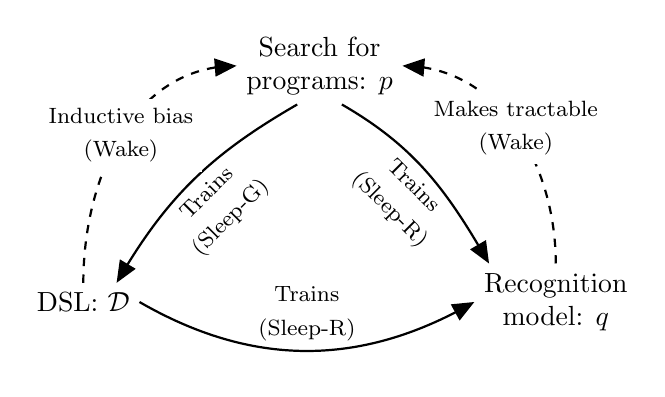
\begin{tikzpicture}
    \begin{scope}[shift = {(1,-1)}]
    \node[align = center](synthesis) at (6,4) {Search for \\programs: $p$};
    \node[align = center](DSL) at (3,1) {DSL: $\mathcal{D}$};
    \node[align = center](recognitionModel) at (9,1) {Recognition \\model: $q$};

    \draw [->,thick] (synthesis.-120) to[out = -150,in = 60] node[below,rotate = 45,align = center]{{\footnotesize Trains}\\{\footnotesize (Sleep-G)}} (DSL.30);
    \draw [->,thick] (synthesis.-60) to[out = -30,in = 120] node[below,rotate=-45,align = center]{{\footnotesize Trains}\\{\footnotesize (Sleep-R)}} (recognitionModel.150);
    \draw [->,thick] (DSL.east) to[out = -30,in = 210] node[above, align = center]{{\footnotesize Trains}\\{\footnotesize (Sleep-R)}} (recognitionModel.west);

    \draw [->,thick,dashed] (DSL.north) to[out = 90,in = 180] node[fill=white,align = center]{  \footnotesize{Inductive bias}\\\footnotesize{(Wake)}} (synthesis.west);
    \draw [->,thick,dashed] (recognitionModel.north) to[out = 90,in = 0] node[fill=white,align = center]{{\footnotesize Makes tractable}\\{\footnotesize (Wake)}} (synthesis.east);
  \end{scope}
    \end{tikzpicture}
  \caption{\system solves for programs, the DSL, and a recognition model. Each of these steps bootstrap off of the others in a Helmholtz-machine inspired wake/sleep inference algorithm.}  \label{feeding}
\end{figure}

Sec.~\ref{mathematicalFraming} frames this 3-step procedure as
a means of maximizing a lower bound on the posterior probability of the DSL given the tasks.
Sec.~\ref{explorationSection} explains how we search for programs that solve tasks;
Sec.~\ref{recognitionSection} explains how we train a neural network to accelerate program search; and
Sec.~\ref{grammarInductionSection} explains how we induce a DSL from programs.

\subsection{Probabilistic Framing}\label{mathematicalFraming}

\system takes as input a set of \emph{tasks}, written $X$, each of which is a program induction problem.
It has at its disposal a \emph{likelihood model}, written $\probability[x|p]$, which scores the likelihood of a task $x\in X$ given a program $p$.
Its goal is to solve each of the tasks by writing a program,
and also to infer a DSL $\mathcal{D}$.

We frame this problem as maximum a posteriori (MAP) inference in the generative model diagrammed by Fig.~\ref{graphicalModel}(a). Writing $J$ for the joint probability of $(\mathcal{D},\theta)$, we want the $\mathcal{D}^*$ and $\theta^*$ solving:
\begin{align}\label{intractableObjectives}
  \nonumber
    J(\mathcal{D},\theta)&\triangleq \probability[\mathcal{D}]\probability[\theta]\prod_{x\in X} \sum_p \probability[x|p]\probability[p|\mathcal{D},\theta]\\
  \mathcal{D}^* &= \argmax_{\mathcal{D}}\int J(\mathcal{D},\theta)\;\mathrm{d}\theta \\
  \nonumber
    \theta^*& =\argmax_\theta J(\mathcal{D}^*,\theta)
\end{align}
The above equations summarize the problem from the point of view of an ideal Bayesian learner.
However, Eq.~\ref{intractableObjectives}
is wildly intractable because evaluating $J(\mathcal{D},\theta)$ involves
summing over the  infinite set of all possible programs.
In practice we will only ever be able to sum over a finite set of programs.
So, for each task, we define a finite set of programs, called a \emph{frontier}, and only marginalize over the frontiers:
\\\noindent\textbf{Definition.} A \emph{frontier of task $x$}, written $\mathcal{F}_x$,
is a finite set of programs where $\probability[x|p] > 0$ for all $p\in \mathcal{F}_x$.

Using the frontiers we  define the following intuitive lower bound on the joint probability, which we call $\lowerBound$:
\begin{align}
 J\geq \lowerBound\triangleq\probability[\mathcal{D}]\probability[\theta]\prod_{x\in X} \sum_{p\in \mathcal{F}_x} \probability[x|p]\probability[p|\mathcal{D},\theta]
\end{align}

%% If we had a $(\mathcal{D},\theta)$ solving Eq.~\ref{intractableObjectives}, then we could recover the most likely program for task $x$ by maximizing $\probability[x|p] \probability[p|\mathcal{D},\theta]$.
%% Through this lens we now take as our goal to solve Eq.~\ref{intractableObjectives}.
%% But even \emph{evaluating} Eq.~\ref{intractableObjectives} is intractable because it involves summing over the infinite set of all possible programs, as an ideal Bayesian learner would.
%% In practice, we must instead marginalize over
%% some finite set of programs.

%% In general, programs are hard-won: finding even a single program that explains a given observation presents a daunting combinatorial search problem.

%% Now in theory we would like to sum over the entire infinite space
%% of all programs -- but this is of course impossible.

%% In general this marginalization over $\theta$ is intractable, so we make an AIC-style approximation\footnote{Sec.~\ref{grammarInductionSection} explains that $\mathcal{D}$ is a context-sensitive grammar.
%% Conventional natural-language processing (NLP) approaches to using variational inference to lower bound the marginal over $\theta$ do not apply in our setting.}, $A\approx \log\probability[\mathcal{D}|X] $:
%% \begin{align}
%%   A =   \log \probability[\mathcal{D}] + \argmax_{\theta}& \sum_{x\in X}\log \sum_p\probability[x|p]\probability[p|\mathcal{D},\theta]\nonumber\\
%% &+  \log P(\theta|\mathcal{D}) - ||\theta||_0 \label{AIC}
%%   \end{align}
\system does approximate MAP inference in the generative model of Fig.~\ref{graphicalModel}(a) by maximizing this lower bound on the joint probability,
alternating maximization w.r.t. the frontiers (Wake) and the DSL (Sleep-G):
%So interleaved with the DSL induction steps are program induction steps. Sec.~\ref{explorationSection}
%explains how \system synthesizes new programs and given a DSL.
\\\noindent \textbf{Program Search: Maxing $\lowerBound$ w.r.t. the frontiers.} Here $(\mathcal{D},\theta)$ is fixed and we
want to find new programs to add to  the frontiers so that $\lowerBound$ increases the most.
$\lowerBound$ most increases by finding programs where $\probability[x,p|\mathcal{D},\theta]$
is large.
%% which we can accomplish by adding new programs to the frontiers means searching for new programs $p$ for task $x$
%% where  is large.
\\\noindent \textbf{DSL Induction: Maxing $\int \lowerBound\;\mathrm{d}\theta$ w.r.t. the DSL.} Here $\left\{\mathcal{F}_x \right\}_{x\in X}$ is held fixed so we can evaluate $\lowerBound$. Now the problem is that of searching the discrete space of DSLs and finding one maximizing $\int \lowerBound\;\mathrm{d}\theta$.
Once we have a DSL $\mathcal{D}$ we can update $\theta$ to $\argmax_\theta \lowerBound(\mathcal{D},\theta,\left\{\mathcal{F}_x \right\})$. 


Searching for programs is hard because
of the large combinatorial search space. We ease this difficulty by training a neural recognition model
during the Sleep-R phase:

\textbf{Neural recognition model: tractably maxing $\lowerBound$ w.r.t. the
  frontiers.}  Here we train a neural network, $q$, to predict a
distribution over programs conditioned on a task. The objective of $q$
is to assign high probability to programs $p$ where
$\probability[x,p|\mathcal{D},\theta]$ is large, because including those programs
in the frontiers will most likely increase $\lowerBound$.  %% With $q$ in hand we can find programs for
%% the frontier $\mathcal{F}_x$ by searching for programs that maximize
%% $q(p|x)$.
Rather than directly predicting a distribution over $p$ conditioned on $x$,
the recognition model predicts a distribution $\theta^{(x)}$ over components of the DSL.
This taps into the intuition that programming is primarily a top-down activity:
as human programmers, we often first decide what kind of
programming constructs we might need to use,
and then we figure out how to assemble them in to the desired program.
%% This approach implements an amortized
%% inference scheme~\cite{le2016inference,ritchie2016deep} for the generative model in
%% Fig.~\ref{graphicalModel}.

Our lower bound $\lowerBound$ is unconventional,
and one might wonder why we do not instead maximize an ELBO-style bound like in a VAE or in the EM algorithm.
We explain in the Supplement that maximizing an ELBO-style bound
leads to a pathological behavior that  causes the model to easily become trapped in local optima.




%% Learning the DSL eases the difficulty of synthesis
%% by exposing a domain-specific basis for constructing programs.
%% Another complementary means of meeting search is to learn a
%% bottom-up \emph{recognition model}

\subsection{Wake Phase: Searching for Programs}\label{explorationSection}

Now our goal is to search for programs that solve the tasks.  In this
work we use the simple search strategy of enumerating programs from
the DSL  in decreasing order of their probability,
and then checking if an enumerated program $p$ assigns positive
probability to a task ($\probability[x|p] > 0$); if so, we include $p$ in
the frontier $\mathcal{F}_x$.

To make this concrete we need to define what programs actually are and
what form $\probability[p |\mathcal{D},\theta]$ takes.
We represent programs as $\lambda$-calculus expressions.
$\lambda$-calculus is a formalism for expressing functional programs
that closely resembles the Lisp programming language.
$\lambda$-calculus includes variables, function application, and the ability to create new functions.
Throughout this paper we will write $\lambda$-calculus expressions in Lisp syntax.
Our programs are all strongly typed.
We use the Hindley-Milner polymorphic typing system~\cite{pierce} which is
used in functional programming languages like OCaml.
Type variables are always written using lowercase Greek letters
and we write $\alpha\to \beta$ to mean a function that takes an input of type $\alpha$
and returns something of type $\beta$.
We use the notation $p:\tau$ to mean that the $\lambda$-calculus expression $p$
has the type $\tau$.
For example, to describe the type of the identity function
we would say \code{(lambda (x) x)}$:\alpha\to \alpha$.
We say a type $\alpha$ \emph{unifies} with $\tau$ if every expression
$p:\alpha$ also satisfies $p:\tau$. Furthermore, the act of \emph{unifying}
a type $\alpha$ with $\tau$ is to introduce constraints on the type
variables of $\alpha$ to ensure that $\alpha$ unifies with $\tau$.
See Supplement for more detail on program representation.
With this notation in hand we now define DSLs:

\noindent\textbf{Definition: $(\mathcal{D},\theta)$.}
A DSL $\mathcal{D}$ is a set of typed $\lambda$-calculus expressions.
%\\\noindent\textbf{Definition.}
A weight vector $\theta$ for a DSL $\mathcal{D}$ is a vector of $|\mathcal{D}| + 1$ real numbers:
one number for each DSL primitive $e\in \mathcal{D}$, written $\theta_e$,
and a weight controlling the probability of a variable occurring in a program, $\theta_{\text{var}}$.

Alg.~\ref{programGenerativeModel} is a procedure for drawing
samples from $\probability[p|\mathcal{D},\theta]$.  In practice, we
enumerate programs rather than sampling them.  Enumeration proceeds by
a depth-first search over the random choices made by
Alg.~\ref{programGenerativeModel}; we wrap the depth-first search
in iterative deepening to build $\lambda$-calculus
expressions in order of their probability.



\begin{algorithm}[tb]
   \caption{Generative model over programs}
   \label{programGenerativeModel}
   \begin{algorithmic}
     \STATE \textbf{function} sampleProgramFromDSL$(\mathcal{D}, \theta, \tau)$:
  \STATE {\bfseries Input:} DSL $\mathcal{D}$, weight vector $\theta$, type $\tau$
  \STATE \textbf{Output:} a program whose type unifies with $\tau$
  \STATE \textbf{return} sample$(\mathcal{D}, \theta, \varnothing, \tau)$
\STATE
     \STATE \textbf{function} sample$(\mathcal{D}, \theta, \mathcal{E}, \tau)$:
  \STATE {\bfseries Input:} DSL $\mathcal{D}$, weight vector $\theta$, environment $\mathcal{E}$, type $\tau$
  \STATE \textbf{Output:} a program whose type unifies with $\tau$
  \IF{$\tau = \alpha\to\beta$}
  \STATE var $\gets$ an unused variable name
  \STATE body $\sim$ sample$(\mathcal{D},\theta,\{\text{var}:\alpha\}\cup\mathcal{E},\beta)$
   \STATE \textbf{return} \code{(lambda (}var\code{) }body\code{)}
   \ENDIF
   %   \ELSE
   \STATE $\text{primitives} \gets\{p | p: \tau' \in \mathcal{D}\cup\mathcal{E}$ \\
     \hspace*{6.9em}$\text{if }\tau\text{ can unify with yield}(\tau') \} $
   
   \STATE Draw $e\sim \text{primitives}$, w.p. $\propto\theta_e$ if $e\in \mathcal{D}$
   \STATE \hspace*{8.8em}w.p. $\propto\frac{\theta_{var}}{|\text{variables}|}$ if $e\in \mathcal{E}$
   \STATE Unify $\tau$ with yield$(\tau')$.
   \STATE $\left\{\alpha_k \right\}_{k = 1}^K\gets\text{argTypes}(\tau')$ 
%   \STATE unify$(\tau,\beta)$
   \FOR{$k=1$ {\bfseries to} $K$}
 \STATE $a_k\sim\text{sample}(\mathcal{D},\theta,\mathcal{E},\alpha_k)$
 \ENDFOR
 \STATE \textbf{return} \code{(}$e\;a_1\; a_2\; \cdots\; a_K$\code{)}
 \STATE\textbf{where:}
 \STATE \quad yield$(\tau) = \begin{cases}
    \text{yield}(\beta)   &\text{ if }\tau = \alpha\to \beta\\
    \tau   &\text{ otherwise.}
 \end{cases}$ 
 \STATE \quad argTypes$(\tau) = \begin{cases}
    [\alpha] + \text{argTypes}(\beta)   &\text{ if }\tau = \alpha\to \beta\\
    []   &\text{ otherwise.}
 \end{cases}$
\end{algorithmic}
\end{algorithm}

Why enumerate, when the program synthesis community has invented many
sophisticated algorithms that search for programs?~\cite{solar2008program,schkufza2013stochastic,feser2015synthesizing,osera2015type,polozov2015flashmeta}.
We have two reasons:
(1) A key point of our work is that learning the DSL, along with a neural recognition model, can make program induction tractable, even if the search algorithm is very simple.
(2) Enumeration is a general approach that can be applied to any program induction problem. Many of these more sophisticated approaches require special conditions on
  the space of programs.

A drawback of using an enumerative search algorithm is that we have no
efficient means of solving for arbitrary constants that might occur in the
program. In Sec.~\ref{regressionSection},
we will show how to find programs with real-valued constants
by automatically differentiating through the program and setting the constants using gradient descent.
%% In Sec.~\ref{textSection}
%% we will show that the bottom-up neural recognition model can learn
%% which discrete constants should be included in a program.







\subsection{Sleep-R: Learning a Recognition Model}\label{recognitionSection}

The purpose of the recognition model is to accelerate the search for
programs.  It does this by learning to predict programs which are probable
under $(\mathcal{D},\theta)$ while also assigning high likelihood for a task
according to $\probability[x|p]$.

The recognition model $q$ is a neural network that predicts,
for each task $x\in X$, a weight vector $q(x) = \theta^{(x)}\in \mathbb{R}^{|\mathcal{D}| + 1}$.
Together with the DSL, this defines a distribution over programs,
$\probability[p|\mathcal{D},\theta = q(x)]$.
We abbreviate this distribution as $q(p|x)$.
The crucial aspect of this framing is that the neural network
leverages the structure of the learned DSL,
so it is \emph{not} responsible for
generating programs wholesale.
We share this aspect with DeepCoder~\cite{balog2016deepcoder}.


We want a recognition model that closely approximates the true posteriors over programs. We formulate this as minimizing the expected KL-divergence, $  \expect\left[\text{KL}\left(\probability[p|x,\mathcal{D},\theta]\|q(p|x) \right) \right]$,
or equivalently maximizing
\begin{equation*}
  \expect\left[\sum_p\probability[p|x,\mathcal{D},\theta]\log q(p|x) \right]
\end{equation*}
where the expectation is taken over tasks. One could take this expectation
over the observed empirical distribution of tasks,
like how an autoencoder is trained~\cite{hinton2006reducing}; or, one could take this expectation over samples from the generative model, like how a Helmholtz machine is trained~\cite{dayan1995helmholtz}.
We found it useful to maximize both an autoencoder-style objective $\mathcal{L}_{\text{AE}}$ and a Helmholtz-style objective $\mathcal{L}_{\text{HM}}$, giving the  objective for a recognition model, $\mathcal{L}_{\text{RM}}$:
\begin{align}
\mathcal{L}_{\text{RM}}& = \mathcal{L}_\text{AE} + \mathcal{L}_\text{HM}\\
\mathcal{L}_{\text{HM}}& = \expect_{p\sim(\mathcal{D},\theta) }\left[\log q(p|x)\right],\text{ $p$ evaluates to $x$}\nonumber\\
\mathcal{L}_{\text{AE}}& = \expect_{x\sim X}\left[\sum_{p\in \mathcal{F}_x}
  \frac{\probability\left[x,p|\mathcal{D},\theta \right]}{\sum_{p'\in \mathcal{F}_x}\probability\left[x,p|\mathcal{D},\theta \right]}\log q(p|x)\right]\nonumber
\end{align}
The $\mathcal{L}_{\text{HM}}$ objective is essential for data efficiency:
all of our experiments train \system on only a few hundred tasks, which is too little for
a high-capacity neural network $q$.
Once we bootstrap a $(\mathcal{D},\theta)$,
we can draw unlimited samples from $(\mathcal{D},\theta)$
and train $q$ on those samples.

Evaluating $\mathcal{L}_{\text{HM}}$ involves sampling programs from
the current DSL, running them to get their outputs,
and then training $q$ to regress from the outputs to the program.
Since these programs map inputs to outputs,
we need some way of sampling these inputs as well.
Our solution to this problem is to sample the inputs
from the empirical observed distribution of inputs in $X$.

The architecture of $q$ depends upon the domain.
For domains with sequential structure like strings and lists,
we use an RNN to encode each input/output example.
For domains with fixed-dimensionality inputs/outputs we use a multilayer perceptron.
We MaxPool across all of the input/output examples. See Supplement for details.

\subsection{Sleep-G: Inducing the DSL}\label{grammarInductionSection}

The purpose of the DSL is to
offer a set of abstractions
that allow an agent to easily express solutions to the tasks at hand.
In the \system algorithm we infer the DSL from a collection of frontiers.
Intuitively, we want the algorithm to
look at  the frontiers and
generalize beyond them, 
both so the DSL can better express the current solutions,
and  also so that the DSL might expose new abstractions
which will later be used to
discover more programs.

Recall from Sec.~\ref{mathematicalFraming} that we want the DSL maximizing $\int \lowerBound\;\mathrm{d}\theta$.
We replace this marginal with an AIC approximation, giving the following objective for DSL induction:
\begin{align}
  \nonumber
    \log \probability[\mathcal{D}] + \argmax_{\theta}&\sum_{x\in X}\log \sum_{p\in \mathcal{F}_x}\probability[x|p]\probability[p|\mathcal{D},\theta]\\
  &+ \log \probability[\theta|\mathcal{D}] - \|\theta\|_0 \label{AIC}
  \end{align}

We induce a DSL by searching locally through the space of DSLs,
proposing small local changes to $\mathcal{D}$ until Eq.~\ref{AIC} fails to increase.
The search moves work by introducing new
$\lambda$-expressions into the DSL.
We propose these new expressions by extracting subexpressions from
programs already in the frontier.
These extracted subexpressions
are fragments of the original programs, and can introduce new variables (Fig.~\ref{fragmentExample}),
which then become new functions in the DSL.
The idea of storing and reusing
fragments of expressions comes from Fragment Grammars~\cite{tim} and Tree-Substitution Grammars~\cite{cohn2010inducing}.



We define a prior distribution over DSLs which penalizes the sizes of the $\lambda$-calculus expressions in the DSL, and put a Dirichlet prior over the weight vector:
\begin{align*}
  \probability[\mathcal{D}]&\propto\exp\left(-\lambda\sum_{p\in \mathcal{D}}\text{size}(p) \right)\\
  \probability[\theta|\mathcal{D}]& = \text{Dir}(\theta|\alpha)
\end{align*}
where $\text{size}(p)$  measures the size of the syntax tree of program $p$,
$\lambda$ is a hyperparameter that acts as a regularizer on the size of the DSL,
and $\alpha$ is a concentration parameter controlling the smoothness of the prior over $\theta$.
%Alg.~\ref{grammarInductionAlgorithm} specifies the DSL induction algorithm.

To appropriately score each proposed $\mathcal{D}$ we must reestimate the weight vector $\theta$.
Although this problem may seem 
very similar to estimating the parameters of a probabilistic context free grammar (PCFG),
for which we have effective approaches like the Inside/Outside algorithm~\cite{international2000derivation},
a DSL in \system may be context-sensitive due to the presence of variables
in the programs and also due to the polymorphic typing system.
In the Supplement we derive a tractable MAP estimator for $\theta$.
 

\begin{figure*}
\centering  \begin{tabular}{lll}
    \toprule
    Domain&Example programs in frontiers&Example proposed subexpression\\\midrule
    Circuits&
    \begin{tabular}{l}
      \code{(lambda x (nand x x))}\\
      \code{(lambda x (lambda y (nand x (nand y y))}
    \end{tabular}&
    \code{(nand z z)}\\\midrule
    Strings&
    \begin{tabular}{l}
      \code{(lambda s (+ ',' (index 0 (split ',' s))))}\\
      \code{(lambda s (index 0 (split ' ' s)))}
    \end{tabular}&
    \code{(index 0 (split z s))}\\\bottomrule
  \end{tabular}
  \caption{The DSL induction algorithm proposes subexpressions of programs to add to the DSL.
    These subexpressions are taken from programs in the frontiers (middle column), and can introduce new variables (\code{z} and \code{s} in the right column).} 
  \label{fragmentExample}
\end{figure*}

\subsection{Implementing \system}

Alg.~\ref{mainAlgorithm} describes how we combine program search,
recognition model training, and DSL induction.
We note the following implementation details:
(1) We perform a wake cycle before each of the sleep cycles.
(2) On the first iteration, we do \emph{not} train the recognition model on samples from
the generative model because a DSL has not yet been learned --
we instead train the network to only maximize $\mathcal{L}_{\text{AE}}$.
%% (3) Because the frontiers can grow very large,
%% we only keep around the top $10^4$ programs $p$ in each frontier $\mathcal{F}_x$
%% with the highest likelihood $\probability[x,p|\mathcal{D},\theta]$.
(3) During both DSL induction and neural net training, we calculate Eq.~\ref{AIC} and $\mathcal{L}_{\text{RM}}$
by only summing over the top $K$
programs in $\mathcal{F}_x$ as measured by $\probability[x,p|\mathcal{D},\theta]$ -- we found that $K = 2$ sufficed.
(4) For added robustness, we enumerate programs from both the generative model and the recognition model.

\begin{algorithm}[tb]
   \caption{The \system Algorithm}
   \label{mainAlgorithm}
   \begin{algorithmic}
     \STATE {\bfseries Input:} Initial DSL $\mathcal{D}$, set of tasks $X$, iterations $I$
     \STATE \textbf{Hyperparameters:} Maximum frontier size $F$
     \STATE \textbf{Output:} DSL $\mathcal{D}$, weight vector $\theta$, recognition model $q(\cdot)$
     \STATE Initialize $\theta\gets \text{uniform}$ %, $q_0(\cdot ) = \theta_0$
     \FOR{$i=1$ {\bfseries to} $I$}
     %     \FOR{$x:\tau\in X$}
     \STATE  $\mathcal{F}^{\theta}_x\gets \{p| p\in \text{enumerate}(\mathcal{D},\theta,F)\text{ if }\probability[x|p] > 0\}$
 %    \ENDFOR
     \STATE $q(\cdot )\gets \text{train recognition model to maximize }\mathcal{L}_{\text{RM}}$
     \STATE  $\mathcal{F}^{q}_x\gets\{p|p\in \text{enumerate}(\mathcal{D},q(x),F)\text{ if }\probability[x|p] > 0\}$
     \STATE $\mathcal{D},\theta\gets $induceDSL$(\{\mathcal{F}^{\theta}_x\cup\mathcal{F}^{q}_x\}_{x\in X})$
     %% \STATE Define $Q_x(z) \propto \begin{cases}
     %%   \probability[x|z]\probability[z|\mathcal{D}_i,\theta_i]&x\in \mathcal{F}_x\\
     %%   0&x\not \in \mathcal{F}_x
     %% \end{cases}
      \ENDFOR
 \STATE \textbf{return} $\mathcal{D},\theta,q$
\end{algorithmic}
\end{algorithm}


\section{Experiments}
We first present our experimental results qualitatively,
illustrating the DSLs we
learn.
We then show quantitative results (Sec.~\ref{quantitative})
comparing \system with lesioned versions
of our model that are analogous to prior work.

\subsection{Boolean circuits}
We consider the problem of learning
to build  Boolean circuits out of logic gates.
If we gave our agent the full repertoire of
circuit primitives -- XOR gates, multiplexers, etc. -- this problem would be easy,
and we could use sophisticated symbolic search algorithms like SMT solvers to synthesize circuits.
Instead, we gave \system only a NAND gate,
and tasked it with building a set of 250 random circuits made out of
AND, NOT, and OR gates, along with a multiplexer.
\system observes the input/output truth table of the circuits,
and we define the likelihood 
$  \probability[x|p]\triangleq\indicator\left[p\text{ has  the same truth table as }x \right]$,
where $x$ is a truth table and $p$ a program implementing a circuit.


This experimental setup is an extension of one introduced in the EC algorithm~\cite{Dechter:2013:BLV:2540128.2540316}.
%% For this domain our recognition model is a simple multilayer perceptron 
%% whose inputs are the input/output examples.
\system learns to build these
circuits by creating new subroutines that correspond to
logic gates and multiplexers (Fig.~\ref{multiplexer}).
We will show that the neural recognition model
assists in building these circuits (Sec.~\ref{quantitative}),
suggesting that an agent can glean something about the structure of a circuit just by looking at its truth table.

\begin{figure}\centering
  \begin{circuitikz} \draw
    (0,0) node (x) {$x$}
    (x)++(0,-0.3) node (y) {$y$}
    (y)++(0,-0.5) node (z) {$z$}
    
    (x)++(1.7,-0.14) node[nand port, scale = 0.5] (xy) {}
    (xy) ++ (0,-1) node[nand port, scale = 0.5] (xz) {}
    (xz) ++ (1,0.2) node[nand port, scale = 0.5] (zxz) {}
    (zxz) ++ (1,0.2) node[nand port, scale = 0.5] (m) {}
    (x) -- (xy.in 1)
    (y) -- (xy.in 2)

    (x) -| (xz.in 1)
    (z.east) -- (xz.in 2)

    (xz.out) -- (zxz.in 2)
    (z.east) |- (zxz.in 1)

    (zxz.out) -- (m.in 2)
    (xy.out) |- (m.in 1)

    (m)++(1.2,0) node (l) {\textsc{MUX}$(x,y,z)$}
    ;
%% (0,0) node[and port] (myand2) {}
%% (2,1) node[xnor port] (myxnor) {}
%% (myand1.out) -- (myxnor.in 1)
%% (myand2.out) -- (myxnor.in 2);
  \end{circuitikz}
  \begin{circuitikz} \draw
    (0,0) node (a) {$a$}
    (a)++(0,-0.7) node (b) {$b$}

    
    (a)++(1,-0) node[nand port, scale = 0.5] (ab1) {}
    (b)++(1,-0) node[nand port, scale = 0.5] (ab2) {}
    (ab1)++(1,-0.35) node[nand port, scale = 0.5] (o) {}

    (a.east) -| (ab1.in 1)
    (a.east) -| (ab1.in 2)
    (b.east) -| (ab2.in 1)
    (b.east) -| (ab2.in 2)

    (ab1.out) -- (o.in 1)
    (ab2.out) -- (o.in 2)

    (o)++(0.8,0) node (l) {\textsc{OR}$(a,b)$}
    ;
  \end{circuitikz}
  \begin{circuitikz}     \node(m)[draw] at (1,-1) {MUX}; \draw
    (0,0) node (w) {$w$}
    (w)++(0,-0.5) node (x) {$x$}
    (x)++(0,-0.5) node (y) {$y$}
    (y)++(0,-0.5) node (z) {$z$}

    (z.east) -| (m.south)
    (y.east) -| (m.west)
    (x.east) -| (m.north)

    
    (y)++(2.5,0.13) node[or port, scale = 0.5] (z) {}
    (m.east) -- (z.in 2)
    (w.east) -| (z.in 1)
    ;
  \end{circuitikz}
\caption{\system discovers multiplexers (above) and OR gates (bottom left), which it uses to make more complicated circuits (bottom right) that it was unable to build without discovering these new primitives.}\label{multiplexer}
  \end{figure}


%% \begin{figure}
%%   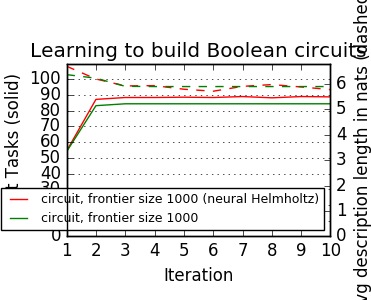
\includegraphics[width = \columnwidth]{figures/circuit.png}
%%   \caption{\system learning to build Boolean circuits. We start out with only NAND gates and learn DSL that contains ...}\label{circuitLearningCurve}
%% \end{figure}



\subsection{Symbolic Regression}\label{regressionSection}
We show how to use \system to infer programs containing both discrete
structure and continuous parameters. The high-level idea is to write programs with unspecified real-valued parameters, and to fit those parameters by differentiating through the program
and optimizing using gradient descent.
We have the algorithm 
solve a set of 200 symbolic regression problems, each a polynomial of
degree 1 to 4, where our observations $x$ are 10
input/output examples.%, which we write as $x = \left\{(i_n,o_n)
%\right\}_{n\leq N}$. %% For example, one task is to infer a program
%% calculating $3x + 2$, and the observations are the input-output
%% examples $\left\{(-1,-1),(0,2),(1,5) \right\}$.

We initially give our system only addition and multiplication,
along with the possibility of introducing real-valued parameters, which we write as $\mathcal{R}$.
We define the likelihood of an observation $x$ by assuming a Gaussian noise model for the input/output examples,
and penalize continuous degrees of freedom using the BIC~\cite{Bishop:2006:PRM:1162264}.
%% \begin{align*}
%%   \log \probability[x|p] \triangleq& \sum_{n\leq N}\log
%%   \mathcal{N}(p(i_n,\vec{\mathcal{R}}^*)|o_n) - \frac{D\log N}{2}
%% \end{align*}

%% %% and integrate over the real-valued parameters, which we collectively write as $\vec{\mathcal{R}}$:
%% %% \begin{align*}
%% %% \log   \probability\left[\{(i_n,o_n)\}|p\right] = \log \int \mathrm{d}\vec{\mathcal{R}}\; P(\vec{\mathcal{R}})\prod_{n\leq N}\mathcal{N}(p(i_n,\vec{\mathcal{R}})|o_n)
%% %% %\text{\emph{BIC:}} &\approx 
%% %% \end{align*}
%% where $\mathcal{N}(\cdot |\cdot )$ is the normal density and
%% $P_{\vec{\mathcal{R}}}(\cdot )$ is a prior over
%% $\vec{\mathcal{R}}$. We approximate this marginal using the BIC~:

%% where $\vec{\mathcal{R}}^*$ is an assignment to $\vec{\mathcal{R}}$
%% found by performing gradient ascent on the likelihood of the
%% observations w.r.t. $\vec{\mathcal{R}}$.

What DSL does \system learn?
The learned DSL contains templates for polynomials of different orders,
which lets the algorithm quickly hone in on the kinds of functions that are most appropriate to this domain (Tbl.~\ref{regressionDSL}).
Examining the programs themselves,
one finds that the algorithm discovers representations for each of the polynomials that minimizes the number of continuous degrees of freedom.
For example, it represents the linear function $-x+2$ with the program
\code{(* (* (+ x }$\mathcal{R}$\code{) }$\mathcal{R}$\code{) x)} which has two continuous degrees of freedom, and represents quartic functions using the invented DSL primitive $f_6$ in Tbl.~\ref{regressionDSL}
which has five continuous degrees of freedom.
This arises from our Bayesian framing -- both the bias towards shorter programs and the likelihood model's BIC penalty.
\begin{table}\centering
\begin{tabular}{l}
  \toprule
  %% Primitives& $+,\times:\mathbb{R}\to \mathbb{R}\to \mathbb{R}$\\
  %% & $\mathcal{R}:\mathbb{R}$ (real valued parameter)\\\midrule
  %% Observation $x$& $N$ input/output examples: $\left\{(i_n,o_n) \right\}_{n\leq N}$\\
  %% \midrule
  %% Likelihood $\probability[x|p]$& $\propto\exp\left( - D\log N \right)\prod_{n\leq N}\mathcal{N}(p(i_n)|o_n)$
  %% \\\midrule
  $f_0\,=\,$\code{(+ $\mathcal{R}$)}\\
  $f_1($\code{x}$)\,=\,$\code{(* (* (+ x $\mathcal{R}$) $\mathcal{R}$) x)} \\
  $f_2($\code{x}$)\,=\,$\code{(+ $\mathcal{R}$ ($f_1$ x))} \\
  $f_3($\code{x}$)\,=\,$\code{(* x ($f_2$ x))}\\
  $f_4($\code{x}$)\,=\,$\code{($f_0$ ($f_3$ x))}\\
  $f_5($\code{x}$)\,=\,$\code{(* x ($f_4$ x))}\\
  $f_6($\code{x}$)\,=\,$\code{($f_0$ ($f_4$ x))} (\emph{4th order polynomial})
  \\\bottomrule
\end{tabular}
\caption{Some induced DSL primitives for symbolic regression. System starts out with addition, multiplication, and real numbers, and learns to build 4th order polynomials.}\label{regressionDSL}
\end{table}

%% The neural recognition model accelerates inference,
%% but given enough iterations of our algorithm,
%% a lesioned version without the recognition model eventually comes close to catching up (green curves in Fig.~\ref{regressionLearningCurve}; No NN in Tbl.~\ref{regressionComparison}).
%% We compare our model on held-out tasks against 4 baselines (Tbl.~\ref{regressionComparison}).


\subsection{String editing}\label{textSection}
Synthesizing programs that manipulate strings is a classic problem in the
programming languages and AI literatures~\cite{menon2013machine,lau2001programming},
and algorithms that learn string editing programs ship in Microsoft Excel~\cite{gulwani2011automating}.
However, this prior work presumes a ready-made DSL,
expertly crafted to suit string editing.
We show in this experiment that we can instead start out with a
less specialized set of primitives -- close to the string routines provided by Python --
and recover many of the higher-level building blocks that have made these
other system successful.
Tbl.~\ref{textPrimitives} (top) lists the primitive functions provided to \systemEnding.
Absent are any routines for searching for characters, extracting substrings,
or replacing one character with another.
Instead, we provide list/string indexing primitives (\code{slice}, \code{nth}),
basic arithmetic, and functions for splitting a string into a list (\code{split})
or turning a list into a string (\code{join}).
We automatically generated  600 string editing tasks  with 4 input/output examples each (Fig.~\ref{exampleTextProblem}). %, split  75/25 train/test.
At first, \system cannot find any programs that
work at all for most of the tasks.
After three wake/sleep iterations,
it assembles a DSL (Tbl.~\ref{textPrimitives}, bottom) that lets it rapidly explore the space of programs and find solutions to
all of the tasks.



\begin{table}[t]
  \centering
  \begin{tabular}{c}
    String editing primitives\\
    \begin{tabular}{l}
    \toprule
    \code{0}, \code{+1},\code{-1},     \code{""},    \code{","},     \code{" "},    \code{"<"}, \code{">"}  \\
    \code{split}, \code{join}, \code{map}, 
    \code{+}, \code{chr->str}, \code{trim}, \code{nth}\\
    \code{length}, \code{slice},    \code{lower}, \code{upper}, \code{capitalize}
  \\\bottomrule
    \end{tabular}\\
\\    Subset of learned DSL\\
    \begin{tabular}{l}
      \toprule
      $f_0($\code{c}$) \,=\, $\code{(+ (chr->str c))}\\
      $f_1($\code{i$,$c$,$s}$) \,=\, $\code{(+ (nth i (split c s))}\\
        \phantom{$f_1($\code{i$,$c$,$s}$) \,=\, $\code{(+ }}\code{(chr->str c))}\\
      $f_2($\code{s$,$c}$) \,=\, $\code{((}$f_0$\code{ c) (}$f_1$\code{ (1+ 0) c s))} \\
        \hspace{0.5cm}($f_2$: \emph{Extract substring delimited by character})\\
      $f_3($\code{c$,$s}$) \,=\, $\code{(nth (1+ 0) (split c (nth 0 s)))}\\
        \hspace{0.5cm}($f_3$: \emph{2nd substring delimited by character})
    %% $f_0($\code{i,c,s}$) = $    \code{(+ (index i (split c s)) (chr->str c))}\\
    %% $f_1 = $\code{(join "")}
  \\\bottomrule
    \end{tabular}
  \end{tabular}
  \caption{Top: provided string editing primitives. Bottom: some induced DSL primitives.}\label{textPrimitives}
  \end{table}

\begin{figure}
  \centering\begin{tabular}{ll}\toprule
    Input&Output\\\midrule
cqbHT$>$aIKd$<$szW& 	AIKD\\
YBW$>$TIg$<$WSho 	&TIG\\
%DkI$>$DwKI$<$xaPoc& 	DWKI\\
KfvTh$>$Dbl$<$OIJso 	&DBL
    \\\bottomrule
  \end{tabular}
  
  \vspace{0.25cm}
  
  \begin{minipage}{7.5cm}
    $f($\code{s}$) \,=\, $\code{(}$f_3$\code{ (split '>' (upper s)) '<')}
  \end{minipage}
  \caption{A string edit task and the program \system writes for it. $f_3$ is a discovered DSL subroutine, defined in Tbl.~\ref{textPrimitives}}\label{exampleTextProblem}.
  \end{figure}

\subsection{List functions}
Synthesizing programs that manipulate data structures is
a widely studied problem in the programming languages community~\cite{feser2015synthesizing}.
%with applications to computer aided programming~\cite{solar2008program}.
We consider this problem within the context of
learning functions that manipulate lists.
We created 225 Lisp-style list manipulation tasks,
each with 15 input/output examples (Tbl.~\ref{listexamples}).
Our data set is challenging along two dimensions:
many of the functions are very complicated,
and the agent must learn to solve these complicated problems from only 225 tasks.

%% Our list function domain consists of hand-designed concepts from which we
%% sample tasks, so there is no ``ground truth'' formal DSL from which these
%% tasks are generated. Additionally, few of these tasks are concatenative ---
%% many of them represent distinct operations.
%% Tasks in this domain are solved by functions that take as input an integer
%% or a list of integers, and have as output either a Boolean, an integer, a
%% list of Booleans, or a list of integers.  There are 225 tasks in total, some
%% of which are shown in Tbl.~\ref{listexamples}.

We evaluate \system starting from two different initial DSLs, \emph{base} and
\emph{rich}. The base DSL starts with only
low-level primitives such as \code{mapi}, \code{reducei}, and
\code{if}, whereas the rich DSL includes some common structure that can be
built from these such as \code{all}, \code{filter}, \code{slice}, and
\code{index}.
Both are capable of solving all tasks supplied by our dataset.
See Supplement for details on these DSLs.

We found  this domain  difficult to tackle without starting from 
the rich DSL. Our
algorithm, like human learners, requires a spectrum of problems ranging from
easy to hard.
When starting with the base DSL,
we found that there were not enough steppingstones in the curriculum to
get \system off the ground.

%The behavior with the base DSL illustrates this phenomena  because the initial set of
%primitives is not paired with a sufficiently large and graded curriculum.

\begin{table}
\centering
\begin{tabular}{lll}
  \toprule
  Name & Input & Output \\\midrule
  append-4 & [7\, 0\, 2] & [7\, 0\, 2\, 4] \\
  len & [3\, 5\, 12\, 1] & 4 \\
  has-2 & [4\, 5\, 7\, 4] & \code{false} \\
  repeat-2 & [7\, 0] & [7\, 0\, 7\, 0] \\
  drop-3 & [0\, 3\, 8\, 6\, 4] & [6\, 4] \\
  count-head-in-tail & [1\, 2\, 1\, 1\, 3] & 2 \\
  rotate-2 & [8\, 14\, 1\, 9] & [1\, 9\, 8\, 14] \\
  pow-3 & [10\, 4\, 13] & [1000\, 64\, 2197] \\
  keep-mod-5 & [5\, 9\, 14\, 6\, 3\, 0] & [5\, 0] \\
  \bottomrule
\end{tabular}
\caption{Sample tasks from our list function domain. %% We used 15 input/output
  %% examples for each task to reduce ambiguity in the task's function,
  %% ensuring solutions achieve the desired concept.
}
\label{listexamples}
\end{table}

\begin{table}[t]
  \centering
  \begin{tabular}{l}
    \toprule
    $f_0($\code{i$,\ell$}$) \,=\, $\code{(singleton (index i $\ell$))}\\
    \hspace{0.5cm}($f_0$: \emph{Put the $i$-th index into a list})\\
    $f_1($\code{i$,\ell$}$) \,=\, $\code{(++ $\ell$ ($f_0$ i $\ell$))}\\
    \hspace{0.5cm}($f_1$: \emph{Append the $i$-th index})\\
    $f_2($\code{n$,\ell$}$) \,=\, $\code{(any (lambda (x) (= n x)) $\ell$)}\\
    \hspace{0.5cm}($f_1$: \emph{Whether $n$ appears in the list})\\
    $f_3($\code{i$,\ell$}$) \,=\, $\code{(index (negate i) (sort $\ell$))}\\
    \hspace{0.5cm}($f_3$: \emph{Get the $i$-th largest number})\\
    $f_4($\code{n$,\ell$}$) \,=\, $\code{(mapi (lambda (i x) (mod x n)) $\ell$)}\\
    $f_5($\code{k$,\ell$}$) \,=\, $\code{(mapi (lambda (i x) (+ x k)) $\ell$)}\\
    $f_6($\code{k$,$n$,\ell$}$) \,=\, $\code{($f_4$ n ($f_5$ k $\ell$)}\\
    \hspace{0.5cm}($f_6$: \emph{Caesar shift of $k$ in integers modulo $n$})\\
  \bottomrule
  \end{tabular}
  \caption{Some induced primitives for list functions.}\label{listinduced}
\end{table}


\subsection{Quantitative Results}\label{quantitative}

We compare  with four baselines on  held-out tasks:
\\\noindent \textbf{Ours--NN}, which lesions the recognition model.
\\\noindent \textbf{RF/DC}, which holds the generative model $(\mathcal{D},\theta)$ fixed and learns
a recognition model only from samples from the fixed generative model.
This is equivalent to our algorithm with $\lambda = \infty$ (see Sec.~\ref{grammarInductionSection})
and $\mathcal{L}_{\text{RM}} = \mathcal{L}_{\text{HM}}$ (see Sec.~\ref{recognitionSection}).
We call this baseline RF/DC because
this setup is closest to how RobustFill~\cite{devlin2017robustfill} and DeepCoder~\cite{balog2016deepcoder} are trained.
\\\noindent \textbf{PCFG}, which lesions the recognition model, learns $\theta$, and fixes $\mathcal{D}$.
This is equivalent to our algorithm with $q(x) = \theta$ and $\lambda = \infty$,
and is like learning the parameters of a PCFG while not learning any of the structure.
\\\noindent \textbf{Enum}, which does no learning and just enumerates a frontier.
This is equivalent to our first wake cycle.

For each domain,
we are interested both in how many tasks the
agent can solve and how quickly it can find those solutions.
For symbolic regression, we also care about the quality
of the solution, as measured by the likelihood model $\probability[x|p]$,
e.g. did the agent correctly explain a linear function
using two numbers, or did it introduce extraneous parameters?
Tbl.~\ref{baselineComparisons}
compares our model against these baselines.
Our full model consistently
beats the baselines,
and that the recognition model 
consistently increases the number of solved held-out tasks.
Lesioning the recognition model also slows down the convergence of the algorithm,
taking more wake/sleep cycles to reach a given number of tasks solved (Fig.~\ref{learningCurves}).
This supports our view of the recognition model as a way of accelerating the search over programs.

\begin{table}
%% This radically shrinks the table
\tabcolsep=4pt
\renewcommand{\arraystretch}{0.5}
\begin{tabular}{llllll}
  \toprule& Ours&Ours--NN  & RF/DC & PCFG & Enum

  \\\midrule\multicolumn{6}{c}{\emph{Boolean Circuits}}\\\midrule
  \% solved &
  \textbf{84\%} &76\%& 63\%&62\%&62\%\\
  Solve time&  0.9s&  1.1s&1.2s&1.3s&1.3s

  \\\midrule\multicolumn{6}{c}{\emph{Symbolic Regression}}\\\midrule
  \% solved&   \textbf{98\% }&94\%&0.7\%&0\%&2\% \\
  Solve time&  2.7s& 2.8s  &3.6s&--&2.1s\\
  MDL (nats)&   9.3 &11.0&2.3&--&4.6

  \\\midrule\multicolumn{6}{c}{\emph{String Editing}}\\\midrule
  \% solved&\textbf{99\%} &82\% &9\%&24\%&18\%\\
  Solve time&  0.9s&2.2s&2.7s&2.3s&2.4s

  \\\midrule\multicolumn{6}{c}{\emph{List functions (base DSL)}}\\\midrule
  \% solved&\textbf{52\%} &\textbf{52\%} &40\%&44\%&42\%\\
  Solve time&  0.4s&0.7s&1.2s&0.9s&1.0s

  \\\midrule\multicolumn{6}{c}{\emph{List functions (rich DSL)}}\\\midrule
  \% solved&\textbf{86\%} &84\% &60\%&74\%&70\%\\
  Solve time&  0.8s&0.7s&1.0s&1.0s&1.1s
  \\\bottomrule
  \end{tabular}
\caption{\% solved: fraction solved w/ 5 sec timeout. Solve time: averaged over solved tasks. MDL: $-\expect\left[\probability[x|p] \right]$. For domains other than symbolic regression MDL is 0 nats. For symbolic regression MDL is a proxy for \# of continuous degrees of freedom.}\label{baselineComparisons}  \end{table}

\begin{figure}\centering
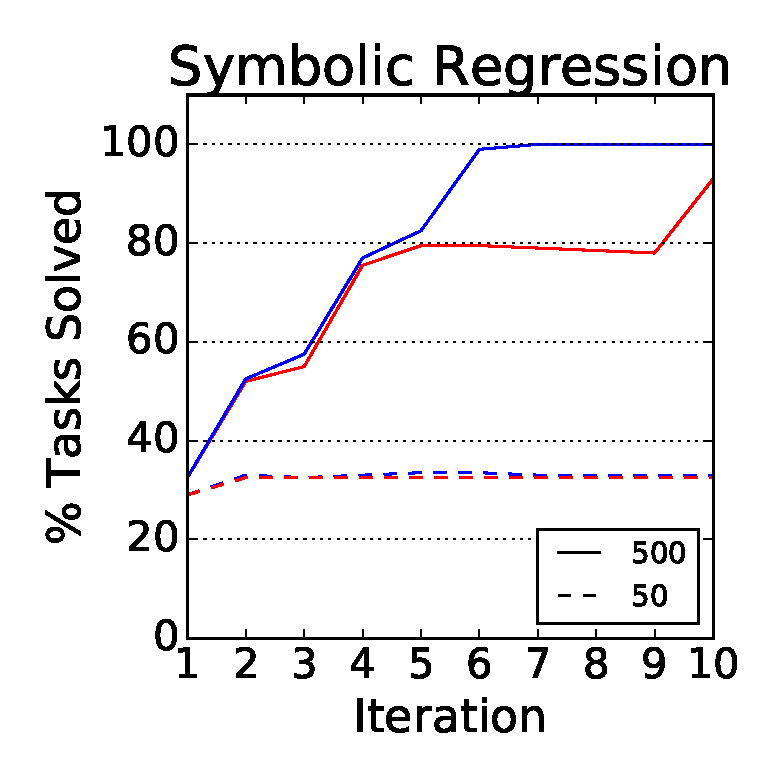
\includegraphics[width = 3.5cm]{figures/regression.eps} 
  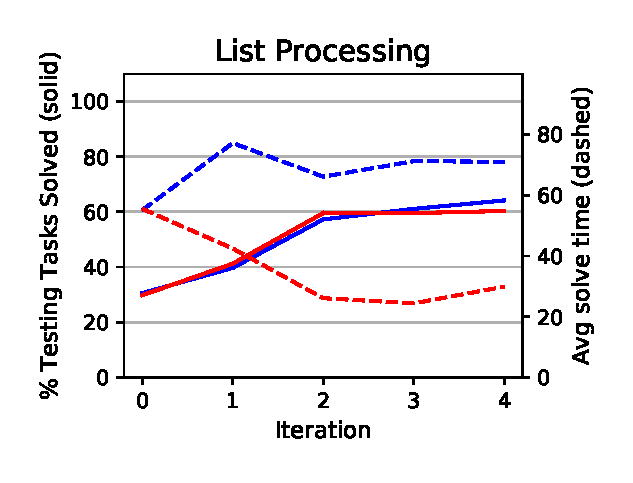
\includegraphics[width = 3.5cm]{figures/list.eps}
  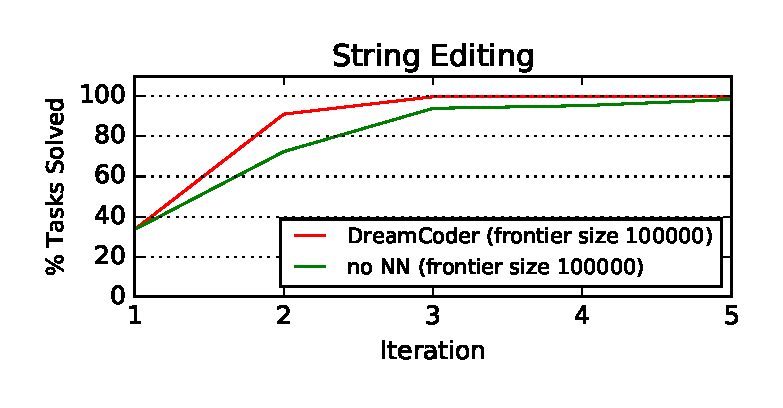
\includegraphics[width = 3.5cm]{figures/textLearningCurve.eps}        
  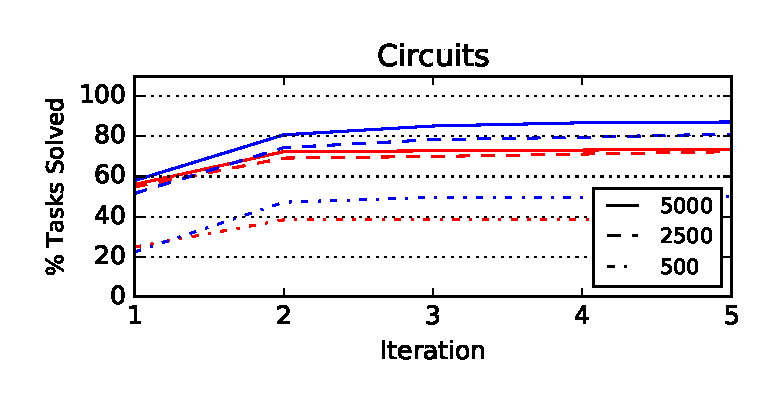
\includegraphics[width = 3.5cm]{figures/circuitLearningCurve.eps}  
  \caption{Learning curves for \system both with (blue) and without (red) the recognition model as the frontier size is varied (solid/dashed/dotted lines).}\label{learningCurves} 
\end{figure}

 \section{Related Work}
 Our work is far from the first to learn to learn programs,
 an  idea that goes back to Solomonoff~\cite{solomonoff1989system}:

 \noindent \emph{Neural recognition models for program induction:} Much recent work in the ML community has
 focused on creating neural networks that regress from
 input/output examples to programs~\cite{devlin2017robustfill,devlin2017neural,menon2013machine,balog2016deepcoder}. This family of work is closest to the lesioned version of
 \system where $(\mathcal{D},\theta)$ is held fixed and $q$ is learned (RF/DC baseline).
 These neural networks are typically trained with strong supervision (i.e., with annotated ground-truth programs) on massive data sets (i.e., hundreds of millions~\cite{devlin2017robustfill}).
 In our work we consider a weakly-supervised setting where ground truth programs are not provided and
 the agent must learn from a few hundred tasks.
 

 \noindent \emph{Inventing new subroutines for program induction:}
 Several program induction algorithms, most prominently the EC algorithm~\cite{Dechter:2013:BLV:2540128.2540316}, take as their goal to learn new, reusable subroutines that are shared in a multitask setting. We find this work inspiring and motivating,
 and extend it along two dimensions: (1) we propose a new algorithm for
 inducing reusable subroutines, based on Fragment Grammars~\cite{tim} and Tree-Substitution Grammars~\cite{cohn2010inducing};
 and (2) we show how to combine these techniques with bottom-up neural recognition models.
 Other instances of this related idea are~\cite{DBLP:conf/icml/LiangJK10}, Schmidhuber's OOPS model~\cite{schmidhuber2004optimal}, and predicate invention in ILP~\cite{DBLP:conf/ecai/LinDETM14}.
 
 Our work is an instance of
 Bayesian Program
 Learning (BPL; see~\citep{lake2013one,Dechter:2013:BLV:2540128.2540316,ellis2016sampling,DBLP:conf/icml/LiangJK10}). Previous BPL systems have largely assumed a fixed DSL (but see~\cite{DBLP:conf/icml/LiangJK10}),
 and our contribution here is a general way of doing BPL with less hand-engineering of the DSL.
 
 \section{Contribution and Outlook}
 We contributed a model, \systemEnding, that learns to program by
 bootstrapping a DSL with new domain-specific primitives that the algorithm itself discovers.
  Alongside this DSL, we train a bottom-up
 neural recognition model that learns how to efficiently deploy the
 DSL and hone in on the right programs.  We believe that this
 integration of top-down symbolic representation and bottom-up neural
 networks -- both of them learned -- is a useful general approach for
 getting program induction off the ground. 
  




\bibliography{main}
\bibliographystyle{icml2018}

\end{document}


% This document was modified from the file originally made available by
% Pat Langley and Andrea Danyluk for ICML-2K. This version was created
% by Iain Murray in 2018. It was modified from a version from Dan Roy in
% 2017, which was based on a version from Lise Getoor and Tobias
% Scheffer, which was slightly modified from the 2010 version by
% Thorsten Joachims & Johannes Fuernkranz, slightly modified from the
% 2009 version by Kiri Wagstaff and Sam Roweis's 2008 version, which is
% slightly modified from Prasad Tadepalli's 2007 version which is a
% lightly changed version of the previous year's version by Andrew
% Moore, which was in turn edited from those of Kristian Kersting and
% Codrina Lauth. Alex Smola contributed to the algorithmic style files.
